\subsubsection{Ý tưởng}
Insertion sort là một thuật toán sắp xếp đơn giản hoạt động bằng cách lặp lại việc chèn từng phần tử của một danh sách chưa được sắp xếp vào đúng vị trí của nó trong một phần đã được sắp xếp của danh sách. Nó giống như việc sắp xếp các lá bài trong tay bạn. Bạn chia các lá bài thành hai nhóm: các lá bài đã được sắp xếp và các lá bài chưa được sắp xếp. Sau đó, bạn chọn một lá bài từ nhóm chưa được sắp xếp và đặt nó vào đúng vị trí trong nhóm đã được sắp xếp.
\subsubsection{Mã giả}

\begin{algorithm}[H]
\caption{Insertion sort}
\begin{algorithmic}[1]
\Procedure{Insertion sort}{$arr, n$}
    \State \textbf{Input:} Mảng $arr$ gồm $n$ phần tử
    \State \textbf{Output:} Mảng $arr$ được sắp xếp
    
    \For{$i \gets 1$ to $n-1$}
    \State $key \gets arr[i]$
    \State $j \gets i - 1$
    \While{$j \geq 0$ \textbf{and} $arr[j] > key$}
        \State $arr[j+1] \gets arr[j]$
        \State $j \gets j - 1$
    \EndWhile
    \State $arr[j+1] \gets key$
\EndFor
\EndProcedure
\end{algorithmic}
\end{algorithm}

\subsubsection{Ví dụ}
Giả sử chúng ta có mảng ban đầu: $[42, 17, 93, 58, 21, 76, 34]$. Dưới đây là các bước thực hiện Insertion sort minh họa bằng hình ảnh:


\begin{figure}[H]
    \centering
    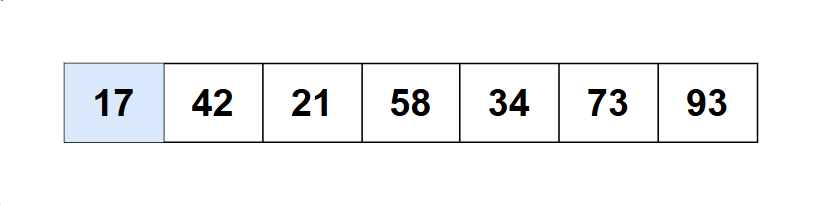
\includegraphics[width=0.7\textwidth]{img/insertion sort_lan2/1.png}
    
\end{figure}

\begin{figure}[H]
    \centering
    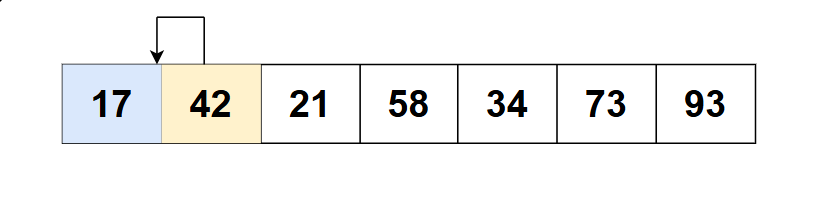
\includegraphics[width=0.7\textwidth]{img/insertion sort_lan2/2.png}
    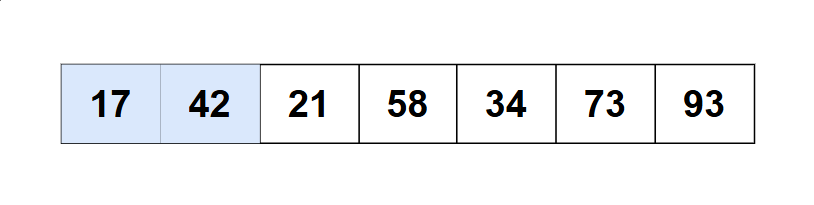
\includegraphics[width=0.7\textwidth]{img/insertion sort_lan2/3.png}
    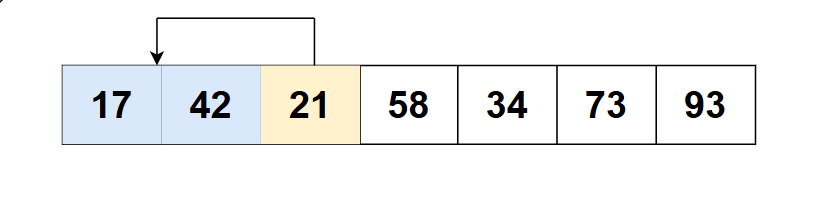
\includegraphics[width=0.7\textwidth]{img/insertion sort_lan2/4.png}
    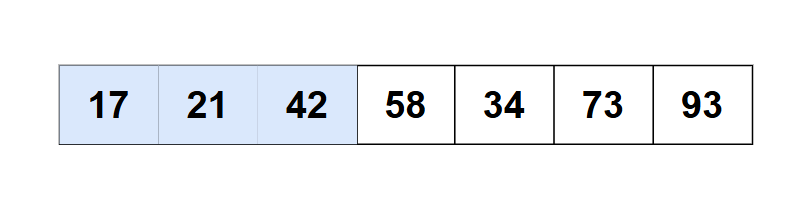
\includegraphics[width=0.7\textwidth]{img/insertion sort_lan2/5.png}
    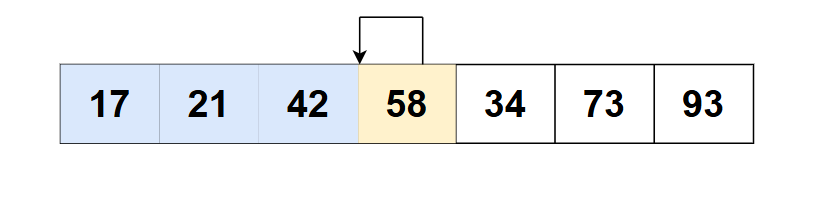
\includegraphics[width=0.7\textwidth]{img/insertion sort_lan2/6.png}
    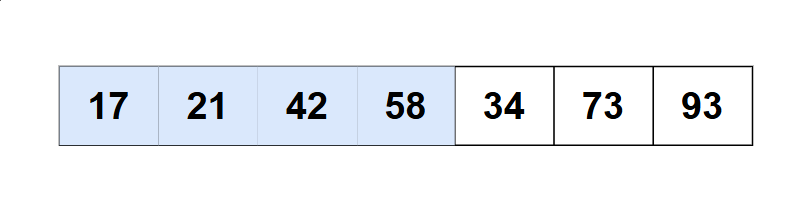
\includegraphics[width=0.7\textwidth]{img/insertion sort_lan2/7.png}
    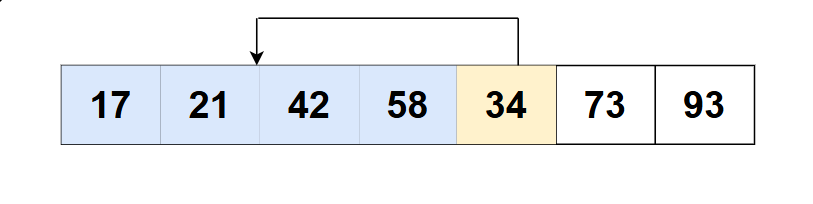
\includegraphics[width=0.7\textwidth]{img/insertion sort_lan2/8.png}
   
\end{figure}

\begin{figure}[H]
    \centering
    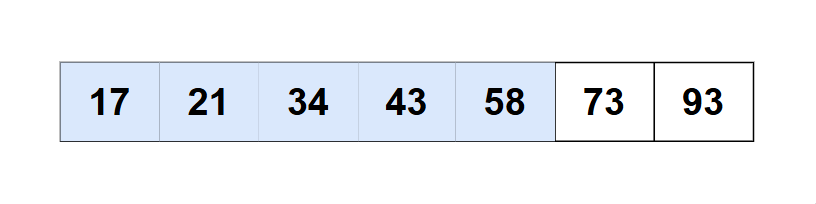
\includegraphics[width=0.7\textwidth]{img/insertion sort_lan2/9.png}
    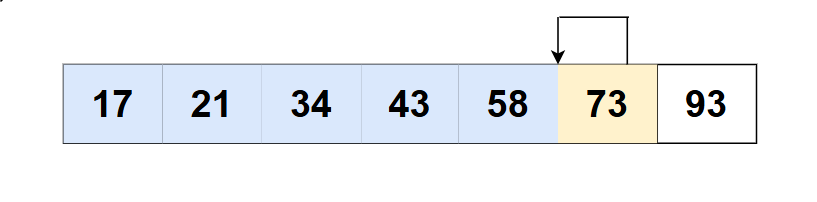
\includegraphics[width=0.7\textwidth]{img/insertion sort_lan2/10.png}
    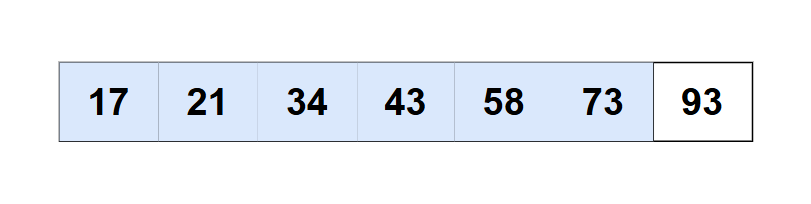
\includegraphics[width=0.7\textwidth]{img/insertion sort_lan2/11.png}
    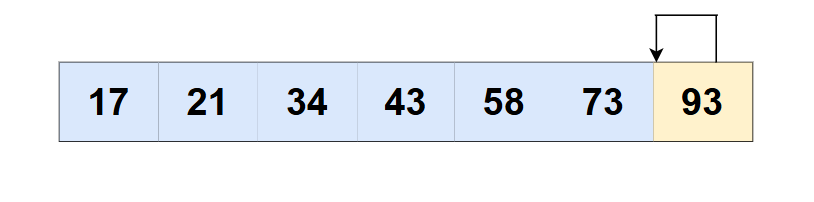
\includegraphics[width=0.7\textwidth]{img/insertion sort_lan2/12.png}
    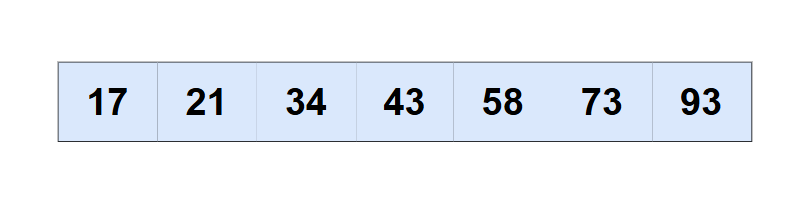
\includegraphics[width=0.7\textwidth]{img/insertion sort_lan2/13.png}

\end{figure}


\subsubsection{Độ phức tạp}
Thuật toán Insertion sort có độ phức tạp thời gian như sau:
\begin{itemize}
    \item Trường hợp tốt nhất: $O(n)$ (mảng đã sắp xếp).
    \item Trường hợp trung bình: $O(n^2)$.
    \item Trường hợp xấu nhất: $O(n^2)$ (mảng sắp xếp ngược).
\end{itemize}